%% Fast markerless drink-task scoring -- IEEEtran conference format
%% Modeled on Unger et al., ICORR 2025 (arXiv:2411.14992).
%%
%% Build:   make            (tectonic, env object_tracking)
%% Tables:  python paper/scripts/make_tables_tex.py   -> tables/*.tex
%% Figures: python paper/scripts/paper_trajectories.py, fig4_correlation.py
\documentclass[conference]{IEEEtran}
\IEEEoverridecommandlockouts

\usepackage{cite}
\usepackage{amsmath,amssymb,amsfonts}
\usepackage{graphicx}
\usepackage{booktabs}
\usepackage{multirow}
\usepackage{siunitx}
\usepackage{xcolor}
\usepackage[hidelinks]{hyperref}
\usepackage{url}

\graphicspath{{./}{figures/}}

% Drafting helpers -- delete before submission.
% \todo = prose still to write. \val = a number NOT yet measured (nothing
% wrapped in \val may survive into a submitted draft).
\newcommand{\todo}[1]{\textcolor{red}{[TODO: #1]}}
\newcommand{\val}[1]{\textcolor{blue}{#1}}

\begin{document}

\title{\todo{title} --- Near Real-Time Markerless Scoring of the\\
Standardized Drinking Task}

\author{\IEEEauthorblockN{Toussaint Foaleng}
\IEEEauthorblockA{\textit{\todo{lab}} \\
\textit{\todo{institution}}\\
\todo{city, country} \\
foaleng@gmail.com}
\and
\IEEEauthorblockN{\todo{co-authors}}
\IEEEauthorblockA{\todo{affiliation}}
}

\maketitle

\begin{abstract}
\todo{Write last, $\sim$200 words. Structure: (1) OMC plus biomechanical
modeling is the reference standard for upper-limb movement quality but is
lab-bound and slow; (2) markerless pipelines have closed much of the accuracy
gap, but the differentiable-biomechanics approach needs days of GPU
optimization per cohort, so results never reach the clinician during the
visit; (3) we present a markerless pipeline --- multi-camera 2D pose, robust
bundle adjustment, temporal smoothing, geometric measure extraction --- that
scores the standardized drinking task within \val{X} of the end of recording
on a single consumer GPU; (4) validated on 11 participants and 697 trials
against synchronized optical mocap, we reach $r_s \ge 0.86$ on six of eleven
Murphy measures and $r \ge 0.96$ on elbow-extension trajectories, without
inverse kinematics; (5) accuracy is comparable to offline markerless work
while running \val{X}$\times$ faster, making same-session feedback feasible.}
\end{abstract}

\begin{IEEEkeywords}
markerless motion capture, optical motion capture, drinking task, movement
quality, stroke rehabilitation, real-time
\end{IEEEkeywords}

\section{Introduction}
\label{sec:intro}

\todo{P1 --- clinical need: stroke prevalence, upper-limb impairment, the case
for frequent objective assessment of movement quality.}

\todo{P2 --- the standardized drinking task and the Murphy measures as the
established instrument~\cite{murphy2011}; OMC plus biomechanical modeling as
the reference standard.}

\todo{P3 --- markerless MMC now approaches OMC accuracy~\cite{unger2024},
removing markers and specialist labor. State the remaining obstacle plainly:
latency. Give the concrete figure --- the end-to-end differentiable pipeline
of~\cite{unger2024} required roughly 12 days of GPU processing for 1160
trials, dominated by 2D keypoint extraction over 5800 videos, plus 30 CPU
hours of OpenSim IK on the OMC side. A result that arrives days later cannot
inform the session that produced it.}

\todo{P4 --- our position. Same task, same measures, same validation protocol,
but every stage chosen so per-trial compute is bounded and overlaps with
recording. Note the deliberate trade: we compute measures geometrically from
3D keypoints rather than fitting a biomechanical model, which costs some
trajectory agreement and buys the latency.}

\paragraph*{Contributions}
\begin{itemize}
  \item A markerless pipeline that produces the Murphy drinking-task
        movement-quality measures in near real time on a single consumer GPU,
        with \todo{a measured per-stage latency budget}.
  \item A validation against synchronized optical mocap on 11 participants and
        697 trials, reporting per-trajectory and per-measure agreement
        (Tables~\ref{tab:trajectories}--\ref{tab:measures}).
  \item \todo{An account of which measures survive the no-IK, geometric
        construction and which do not --- and why the failures are anatomical
        (occluded seated hips) rather than algorithmic.}
\end{itemize}

\section{Related Work}
\label{sec:related}

\subsection{Movement quality assessment in the drinking task}
\todo{Murphy et al.\ measures, clinical use, what each is meant to capture.}

\subsection{Markerless motion capture for clinical kinematics}
\todo{Multi-view pose estimation, triangulation, biomechanical fitting.
Position \cite{unger2024} as the closest comparison: same task, same measures,
OMC-validated --- but offline, and IK-based.}

\subsection{Latency in clinical measurement pipelines}
\todo{Little prior work reports latency at all. Argue that time-to-result is a
first-class metric for clinical adoption, and that reporting accuracy alone
has hidden this axis.}

\section{Methods}
\label{sec:methods}

\subsection{Participants and Task}
\todo{DELTA cohort: 11 participants, both arms, standardized drinking task.
Fill in demographics, impairment scores, ethics approval, repetitions per arm.
State the trial accounting --- 697 trials enter the measure comparison; the
per-frame trajectory comparison (Tables~\ref{tab:trajectories},
\ref{tab:biasiqr}) is computed on the 220-trial subset for which per-frame OMC
trajectories were exported --- and say why, or extend the export.}

\subsection{Data Acquisition}
\todo{Camera rig: number of cameras, model, resolution, frame rate ($60$\,Hz),
geometry, ChArUco calibration, synchronization. OMC system and marker set,
sampling rate ($100$\,Hz). Note the camera-quality auditing that had to
precede any of this --- mis-cut clips and moved cameras, and how they were
detected --- since it bears directly on what a deployable system must
self-check.}

\subsection{Pipeline}
\label{sec:pipeline}
\todo{One paragraph per stage, each stated with its throughput, because cost
is the point of the paper:}
\begin{enumerate}
  \item \emph{2D body pose.} An off-the-shelf YOLO-pose network, run per
        frame on every camera. \todo{state version, input size 640 --- and why
        inference must run at the size the network was trained at --- and the
        fps achieved.}
  \item \emph{Cup localization.} A separate YOLO detector locates the cup
        \emph{once}, at the start of the trial; a transformer visual-object
        tracker (UETrack-B) then follows it through the remaining frames in
        each camera. The cup trajectory is used \emph{only} to segment the
        movement into phases (Sec.~\ref{sec:phases}); no movement-quality
        measure is computed from it. \todo{Motivate detect-once: per-frame
        detection loses the cup at the drinking apex, where it is occluded and
        small --- several 1--3\,s blackouts per trial, falling exactly on the
        phase that defines the segmentation. Detect-once plus tracking fills
        those frames. State that no re-anchoring is used, and why: re-seeding
        from a shared consensus couples the cameras and can cascade them all
        onto the same wrong object, destroying the independence that
        multi-view voting relies on.}
  \item \emph{3D reconstruction.} Robust-reprojection bundle adjustment over
        all nine upper-body joints, Huber loss, no bone-length prior.
        \todo{Say explicitly that a bone-length prior was tested and rejected:
        it rigidifies bone lengths but slides joints along the unobservable
        depth ray, worsening agreement with OMC. Describe the multi-view
        consensus rule used to accept a 3D point.}
  \item \emph{Temporal smoothing.} SmoothNet. \todo{State that smoothing, not
        the reconstruction, is what governs peak-velocity accuracy.}
  \item \emph{Phase segmentation.} From the cup trajectory; see
        Sec.~\ref{sec:phases}.
  \item \emph{Measure extraction.} Geometric, from 3D body keypoints only; see
        Sec.~\ref{sec:measures}.
\end{enumerate}

\subsection{Phase Segmentation}
\label{sec:phases}
\todo{Describe the segmenter: how the cup 3D trajectory yields the
drinking-task phases (speed and displacement-from-rest), and the dwell
definition. This is the only place the cup is used.}

\todo{Keep the two roles of the cup distinct and say so plainly: the
segmentation reported in the deployed pipeline comes from the cup, but the
measure validation in Sec.~\ref{sec:results} deliberately uses the OMC phases
for \emph{both} systems, so that the numbers isolate pose error from
phase-classification error. If segmentation accuracy is to be claimed, it
needs its own comparison against OMC phase boundaries --- reported as boundary
error in seconds, separately from the measure tables.}

\todo{Note on the cup's absolute accuracy, if any cup number is reported: our
centroid is the cup body while the mocap markers sit on the rim, giving a
constant $\approx 60$\,mm offset, and there is a displacement-proportional
$\approx 10\%$ scale error that belongs to the camera calibration, not the
tracker. The latter is not cup-specific --- it inflates every 3D distance and
velocity the pipeline reports, body keypoints included --- so decide whether
it is disclosed here or in Limitations.}

\subsection{Movement Quality Measures}
\label{sec:measures}
\todo{Condense \texttt{measures\_methods.md} into publishable prose. The two
ground rules to state up front: (i) smooth position, then differentiate ---
never filter a raw derivative; (ii) all peak/angle measures are windowed by
phase. Then the constants table (4\,Hz position low-pass, 6\,Hz on the speed
for the peak-velocity operator, 2nd-order zero-phase Butterworth, 60\,mm/s
movement-unit amplitude, 0.15\,s gap) and the geometric definition of each
angle. Justify the three choices that are non-obvious and were empirically
forced: peak velocity uses the differentiate-then-low-pass operator and is
scoped to reaching; trunk displacement is a 3D excursion of the shoulder
midpoint rather than an anatomical forward projection, because the forward
normal depends on occluded seated hips; shoulder flexion uses a per-trial
constant trunk-down axis for the same reason.}

\todo{Also state which measures are not reported and why: the two
percent-timing variants (redundant once phase duration is shared), and
drinking-phase shoulder flexion (no ground-truth column exists), giving 11
panels rather than 12.}

\subsection{Latency Model}
\label{sec:latency}
\todo{THIS SECTION IS THE PAPER'S NOVELTY AND IS NOT YET MEASURED. Define
precisely what is timed --- wall-clock from the last recorded frame of a trial
to its scored output --- and decompose it per stage. Separate streaming cost,
which overlaps with recording, from tail cost, which can only start once the
trial ends; the headline claim is a bound on the tail. Specify the hardware
and state whether recording and inference share the GPU. Make the definition
reproducible enough that another group can time their own pipeline the same
way.}

\subsection{Validation Protocol}
\label{sec:validation}
All measures are computed from our markerless keypoints alone; the optical
system's processed output is read only as the value to compare against and
never enters our computation.
\todo{Spatial and temporal alignment to OMC; time lag from wrist-speed
cross-correlation; static-bias handling. Per-trajectory agreement as $r$,
RMSE, bias and lag; per-measure agreement as Spearman $r_s$ across trials and
$r_{av}$ on per-participant, per-arm averages. State that correlations are
computed within-arm and never pooled across affected and unaffected arms,
since pooling would inflate $r$ with the between-arm difference.}

\todo{Important framing point to make here, not buried in Discussion: for a
measure whose OMC values are near-constant across a cohort, a rank correlation
has little true variance to track and reads low even when the two systems
agree. Report such measures as agreement (fraction of trials within a
tolerance, plus bias), and check the OMC-side effect size before drawing any
conclusion from a low $r$.}

\section{Results}
\label{sec:results}

\subsection{Study Population}
\todo{Table: demographics, impairment scores, trial counts, exclusions with
reasons. 826/837 recorded repetitions were scorable.}

\subsection{Latency}
\label{sec:results-latency}
\todo{Table: per-stage wall-clock, streaming versus tail, total
time-to-result, and the hardware. Compare against the offline baseline
normalized to the same trial count. NOT YET MEASURED --- this table does not
exist and is the main gap between the current results and the paper's claim.}

\subsection{Kinematic Trajectory Agreement}
Table~\ref{tab:trajectories} reports per-frame agreement for the six
kinematic trajectories, and Table~\ref{tab:biasiqr} the within-participant
variability of the static bias. Fig.~\ref{fig:trajectories} shows exemplary
trajectories for one participant.
\todo{Prose: elbow extension and shoulder flexion agree closely; the velocity
trajectories sit near $r=0.75$; shoulder abduction on the unaffected arm is
the weakest. Say what the bias columns mean --- a consistent offset is
correctable, a variable one is not, which is what Table~\ref{tab:biasiqr}
addresses.}

\begin{table}[t]
\caption{Medians and [IQRs] across trials for the six kinematic trajectories, by arm.
Bias is markerless minus optical and is removed before RMSE; the Bias IQR row is the
mean across participants of each participant's own IQR of it.}
\label{tab:trajectories}
\centering
\scriptsize
\setlength{\tabcolsep}{3pt}
\begin{tabular}{llcc}
\toprule
Kinematic & Value & Unaffected arm & Affected arm \\
\midrule
End-effector vel. & $r$ & 0.98 [0.98, 0.99] & 0.98 [0.97, 0.98] \\
 & RMSE (mm/s) & 37.01 [28.76, 45.03] & 42.51 [33.68, 48.42] \\
 & Bias (mm/s) & -5.68 [-8.62, -1.69] & -8.91 [-12.59, -3.65] \\
 & Bias IQR (mm/s) & 4.54 & 4.76 \\
\midrule
Elbow ang.\ vel. & $r$ & 0.97 [0.96, 0.98] & 0.96 [0.95, 0.97] \\
 & RMSE (deg/s) & 11.70 [9.79, 13.90] & 11.84 [10.07, 13.63] \\
 & Bias (deg/s) & 4.03 [3.01, 5.06] & 3.84 [2.67, 5.59] \\
 & Bias IQR (deg/s) & 1.17 & 1.11 \\
\midrule
Elbow extension & $r$ & 1.00 [0.99, 1.00] & 1.00 [0.99, 1.00] \\
 & RMSE (deg) & 4.16 [3.65, 4.73] & 4.24 [3.24, 5.15] \\
 & Bias (deg) & 7.44 [4.61, 8.98] & 8.08 [3.05, 11.07] \\
 & Bias IQR (deg) & 1.08 & 1.06 \\
\midrule
Shoulder flexion & $r$ & 0.96 [0.92, 0.98] & 0.97 [0.93, 0.98] \\
 & RMSE (deg) & 3.26 [2.59, 4.07] & 2.96 [1.65, 3.97] \\
 & Bias (deg) & -5.04 [-8.78, -3.47] & -3.17 [-5.99, -0.91] \\
 & Bias IQR (deg) & 1.17 & 1.07 \\
\midrule
Shoulder abduction & $r$ & 0.78 [0.62, 0.91] & 0.88 [0.77, 0.94] \\
 & RMSE (deg) & 2.33 [1.79, 4.16] & 2.19 [1.74, 3.06] \\
 & Bias (deg) & -5.98 [-7.95, -2.88] & -1.95 [-7.33, 0.09] \\
 & Bias IQR (deg) & 0.84 & 0.94 \\
\midrule
Trunk displacement & $r$ & 0.96 [0.89, 0.98] & 0.98 [0.94, 0.99] \\
 & RMSE (mm) & 3.96 [3.14, 6.11] & 4.50 [3.73, 6.77] \\
 & Bias (mm) & 1.68 [-0.50, 3.67] & 0.71 [-2.70, 4.06] \\
 & Bias IQR (mm) & 2.81 & 2.77 \\
\bottomrule
\end{tabular}
\end{table}

\begin{table}[t]
\caption{Mean IQR of the static bias across participants, i.e.\ the
within-participant trial-to-trial variability of the offset between MMC and OMC.}
\label{tab:biasiqr}
\centering
\scriptsize
\begin{tabular}{lcc}
\toprule
Kinematic & Unaffected arm & Affected arm \\
\midrule
End-effector velocity (mm/s) & 4.54 & 4.76 \\
Elbow angular velocity (deg/s) & 1.17 & 1.11 \\
Elbow extension (deg) & 1.08 & 1.06 \\
Shoulder flexion (deg) & 1.17 & 1.07 \\
Shoulder abduction (deg) & 0.84 & 0.94 \\
Trunk displacement (mm) & 2.81 & 2.77 \\
\bottomrule
\end{tabular}
\end{table}


\begin{figure}[t]
  \centering
  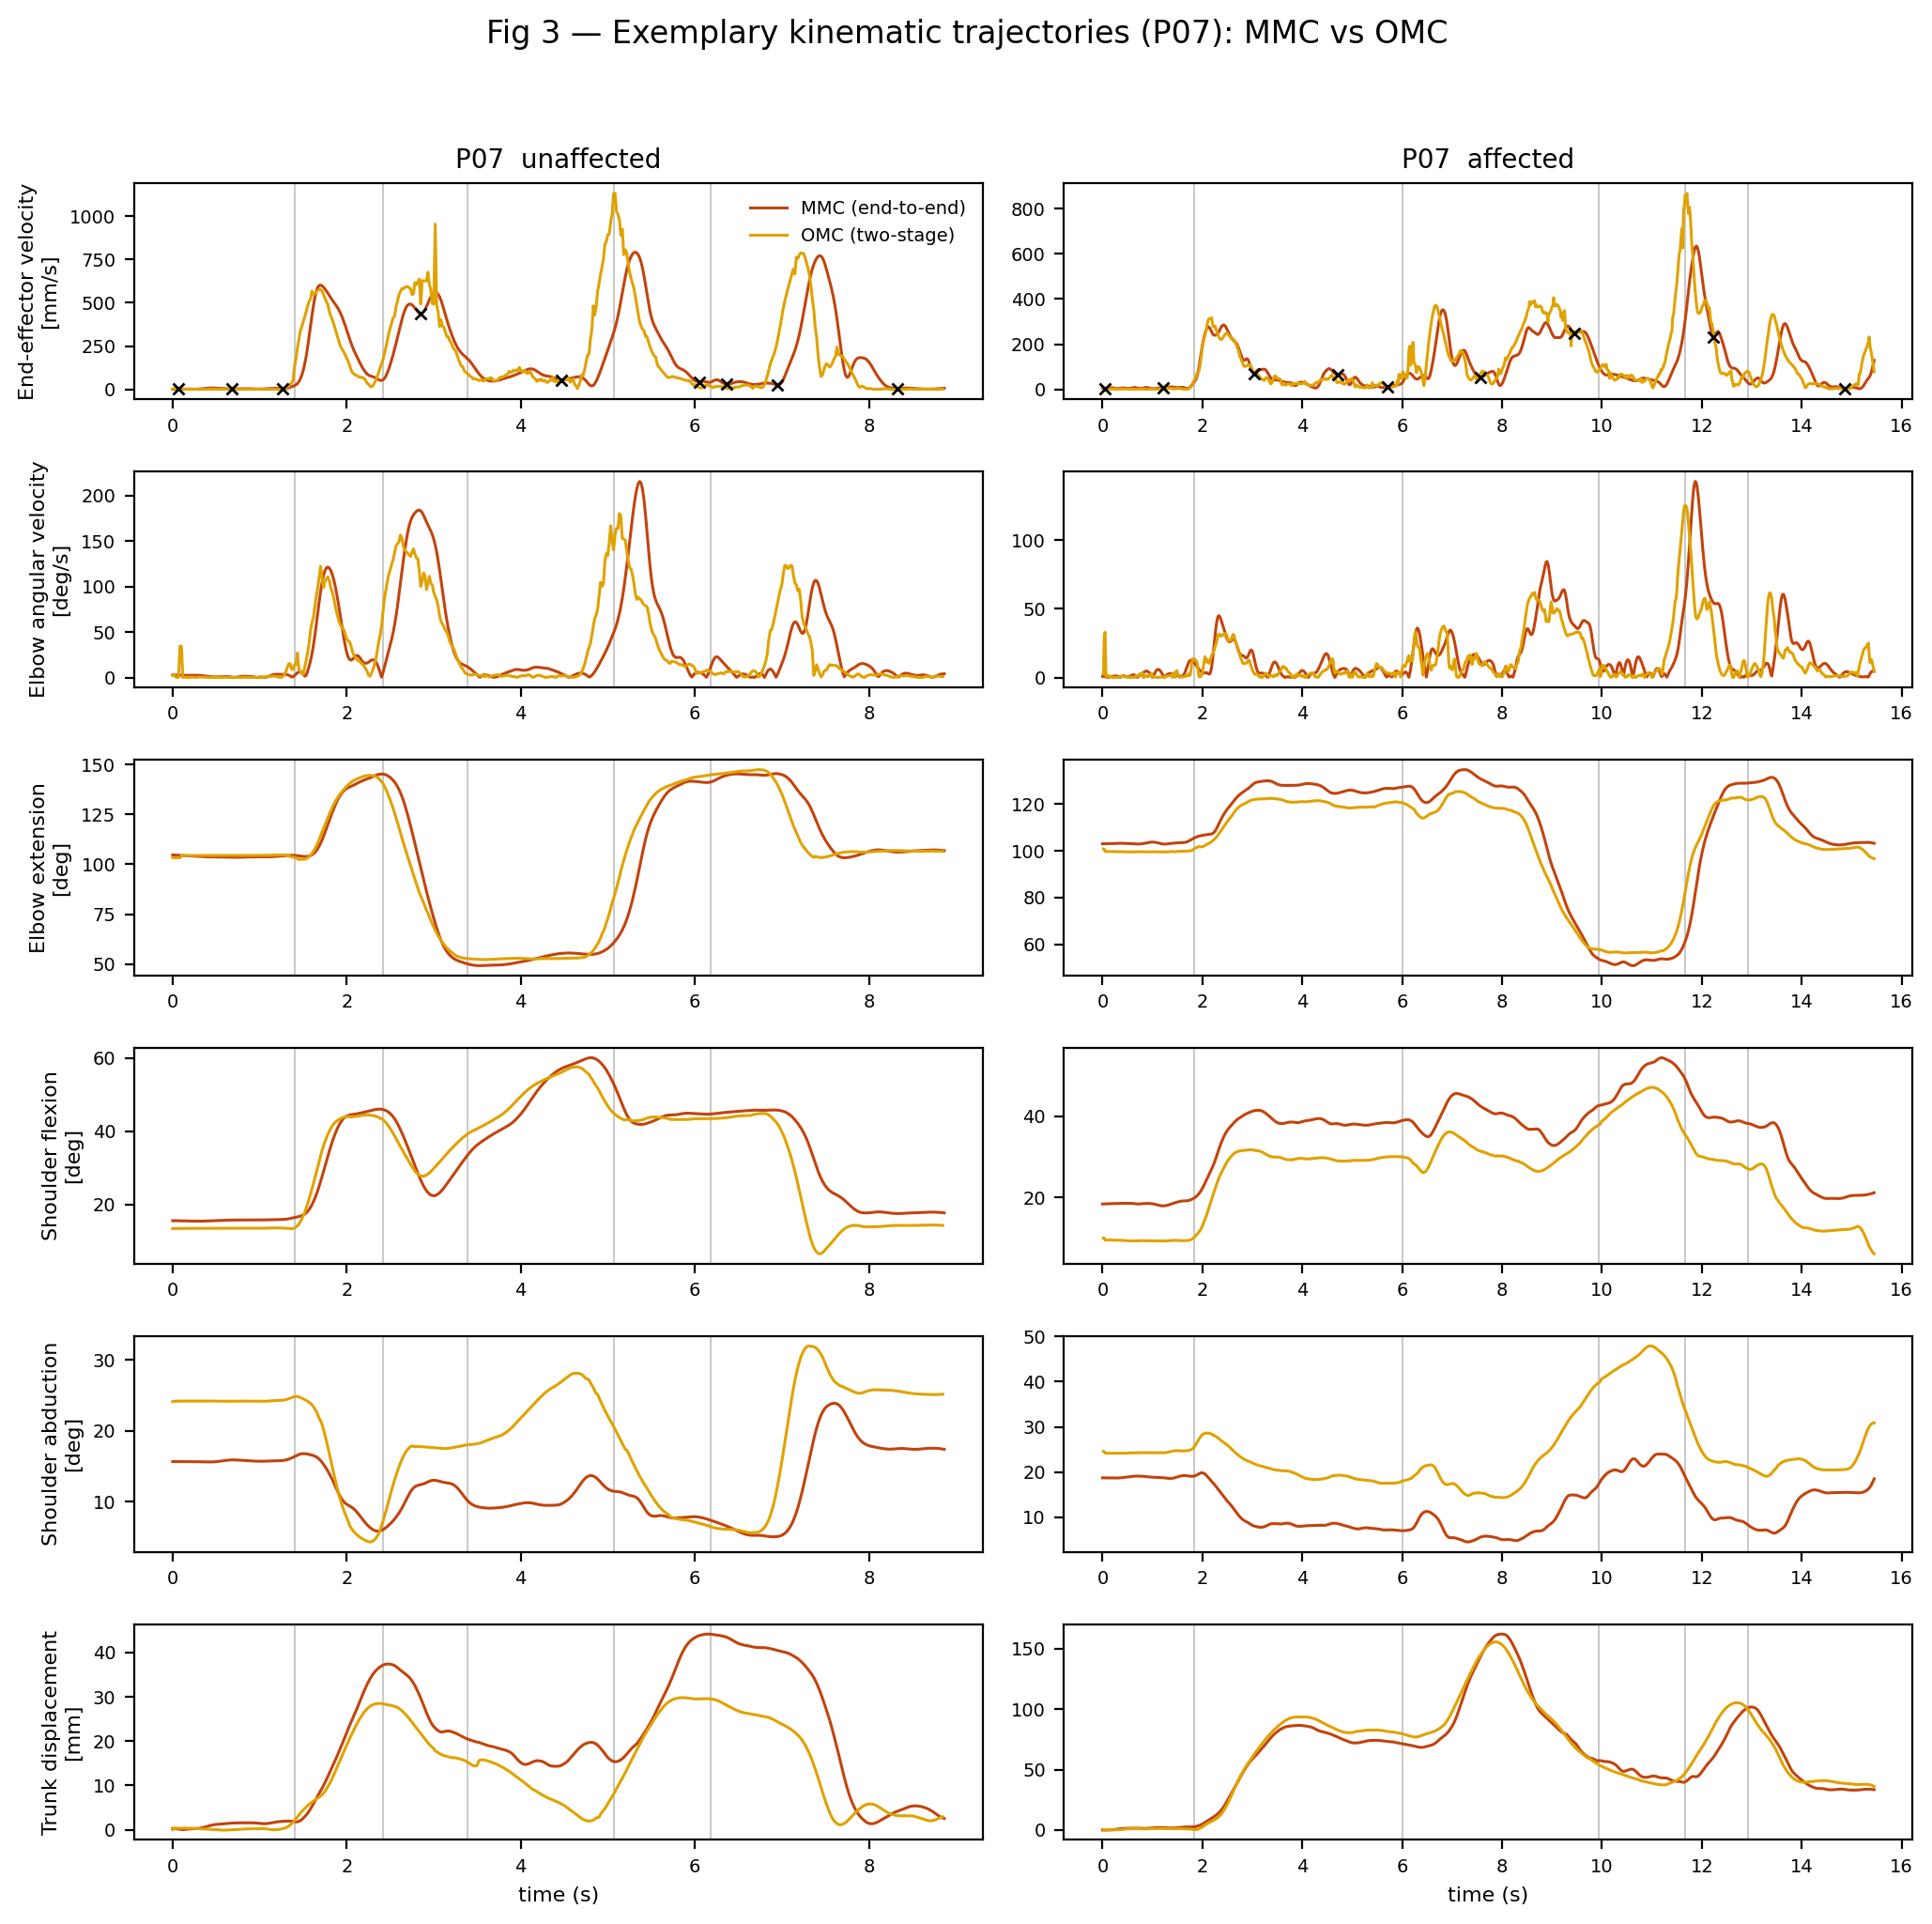
\includegraphics[width=\linewidth]{fig3_trajectories.png}
  \caption{Exemplary kinematic trajectories for the affected and unaffected
  arm, MMC versus OMC, with drinking-task phases marked and movement units
  indicated on the end-effector velocity. \todo{name participant and trials}}
  \label{fig:trajectories}
\end{figure}

\subsection{Movement Quality Measures}
Table~\ref{tab:measures} and Fig.~\ref{fig:correlation} report agreement for
the eleven movement-quality measures.
\todo{Prose: six measures reach $r_s \ge 0.86$. Total movement time is
phase-derived and, because both systems share OMC phases here, is near
tautological at $r_s = 1.00$ --- report it as a consistency check, not as
validation of pose. Number of movement units and interjoint coordination are
intrinsically noisy; shoulder flexion is limited by the occluded seated-hip
keypoint. Be explicit that these are floors of the construction, not of the
reconstruction.}

\begin{table}[t]
\caption{Movement-quality measures: Spearman correlation between MMC and OMC
across all trials ($r_s$) and on per-participant, per-arm averaged trials ($r_{av}$).}
\label{tab:measures}
\centering
\footnotesize
\begin{tabular}{lccc}
\toprule
Movement quality measure & $r_s$ & $r_{av}$ & $n$ \\
\midrule
PV [mm/s] & 0.87 & 0.93 & 697 \\
Elbow angular PV [deg/s] & 0.80 & 0.77 & 695 \\
Time to PV [s] & 0.93 & 0.93 & 697 \\
Time to first PV [s] & 0.90 & 0.94 & 697 \\
Number of movement units [n] & 0.53 & 0.72 & 697 \\
Total movement time [s] & 1.00 & 1.00 & 697 \\
Interjoint coordination & 0.48 & 0.66 & 695 \\
Trunk displacement [mm] & 0.92 & 0.94 & 695 \\
Shoulder flexion [deg] & 0.26 & 0.19 & 695 \\
Elbow extension [deg] & 0.90 & 0.88 & 695 \\
Shoulder abduction [deg] & 0.70 & 0.68 & 695 \\
\bottomrule
\end{tabular}
\end{table}


\begin{figure}[t]
  \centering
  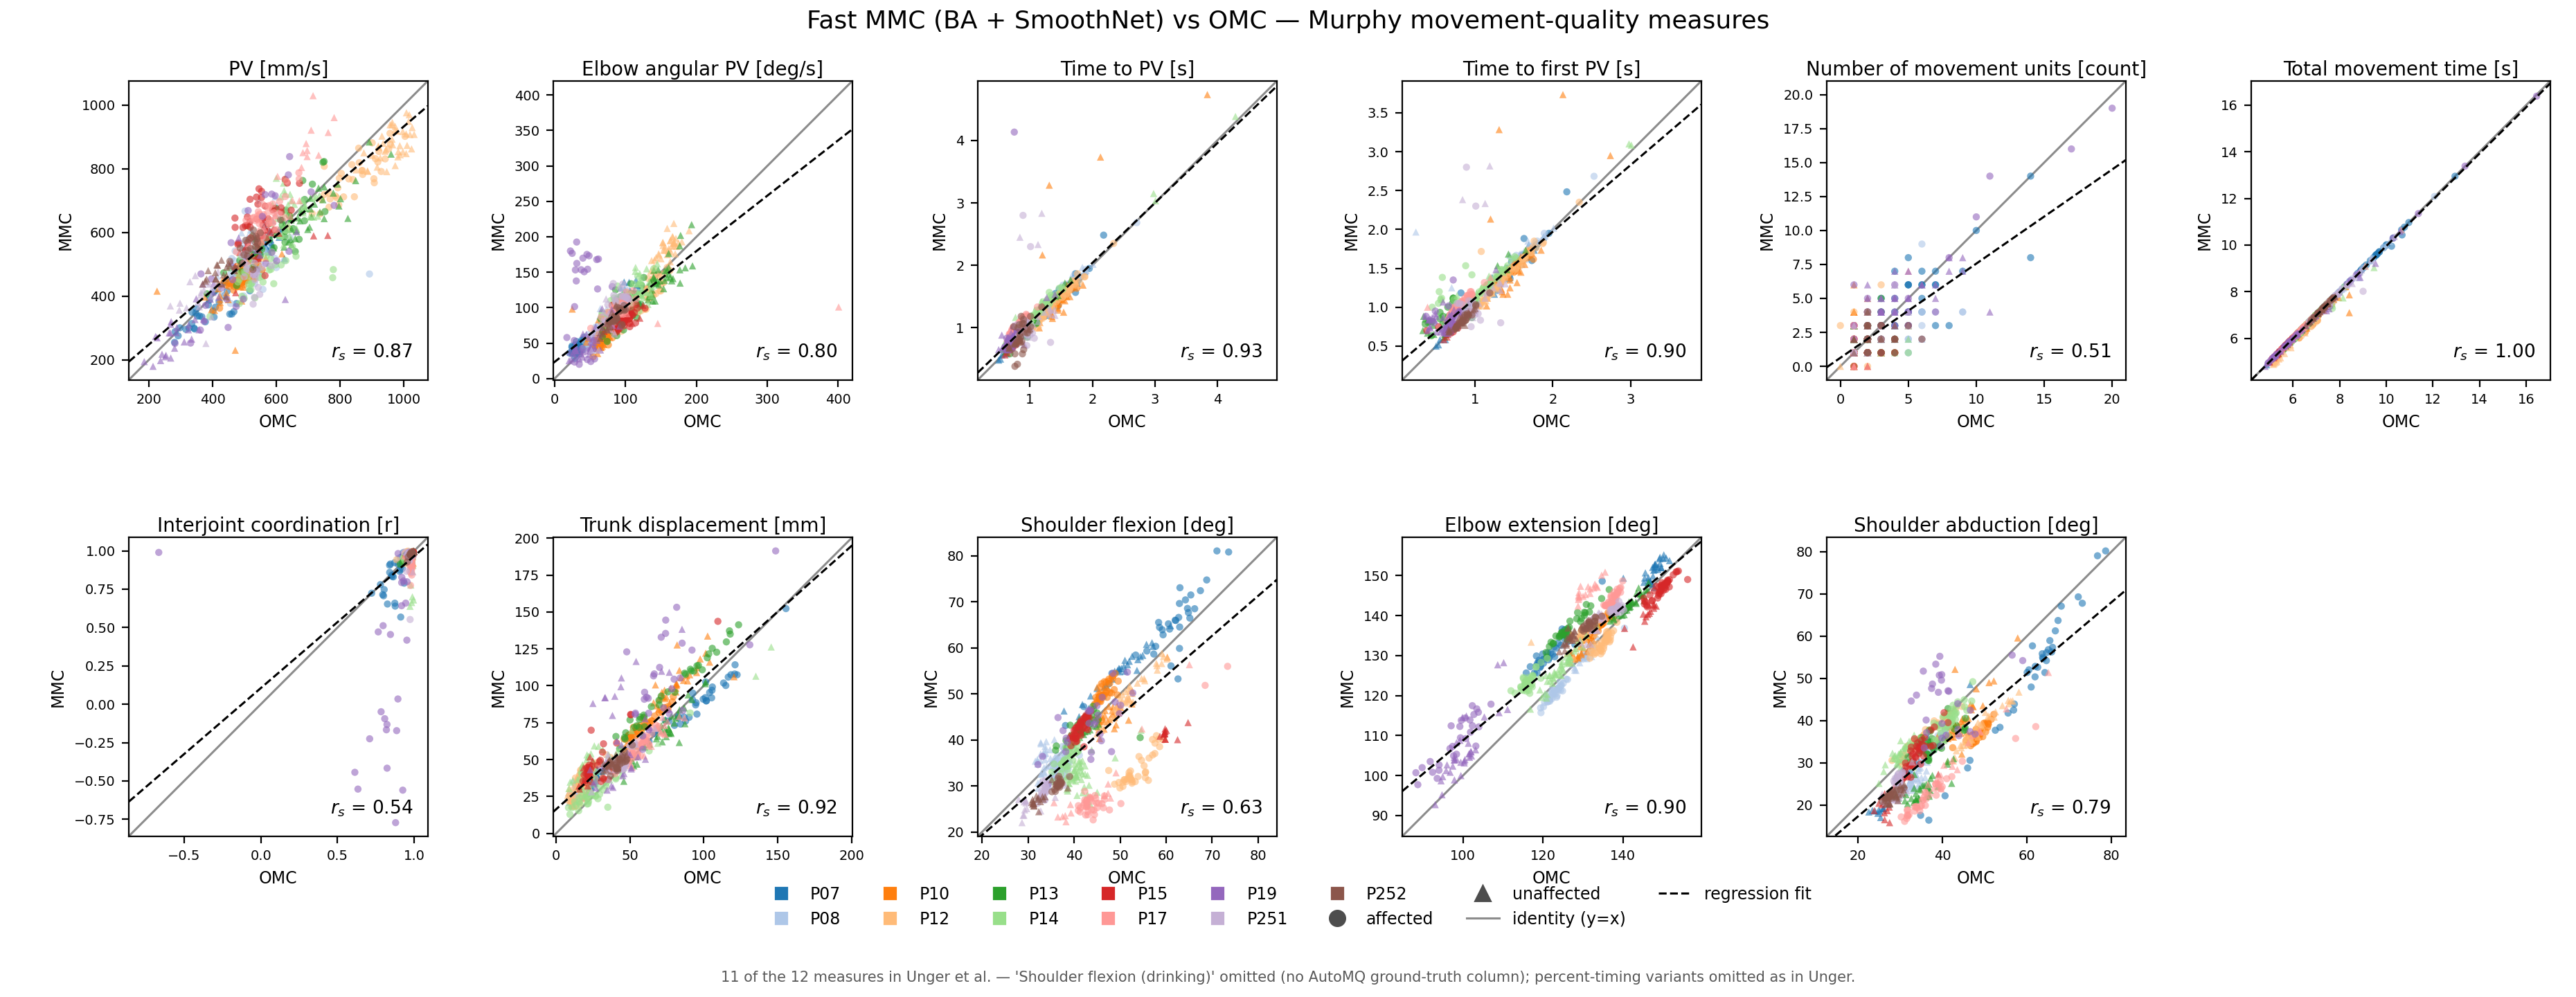
\includegraphics[width=\linewidth]{fig4_mmc_vs_omc.png}
  \caption{Movement-quality measures, MMC versus OMC, per participant and
  arm. Eleven measures; see Sec.~\ref{sec:measures} for the two omitted by
  construction.}
  \label{fig:correlation}
\end{figure}

\subsection{Ablations}
\todo{What each accelerated or simplified component costs in accuracy.
Material already exists for: bundle adjustment with and without the bone-length
prior; smoothing on and off; camera-dropout and miscalibration augmentation
(\texttt{augment*.csv}); segmentation factors (\texttt{seg\_factors.csv}).
Select rather than dump --- one table of the choices a reimplementer must get
right.}

\section{Discussion}
\label{sec:discussion}
\todo{What the numbers support and what they do not. Our trajectory
correlations sit a notch below IK-based markerless work (elbow extension
$r \approx 0.96$ versus $0.99$) --- same ordering, similar ballpark, from
consumer webcams at 60\,Hz with no biomechanical model, and fast enough to
report during the session. Where the residual error lives: the weakest
measures are limited by occluded seated anatomy, which is a camera-placement
and modeling issue rather than a detector one. Clinical implication of
same-session feedback.}

\section{Limitations}
\todo{Cohort size and composition; single site; the trajectory subset noted in
Methods; dependence on camera placement and calibration quality, including
that some sessions required re-cutting or recalibration before they were
usable; measures that could not be validated for lack of a ground-truth
column; and that geometric angles are not anatomical joint angles.}

\section{Conclusion}
\todo{Two or three sentences.}

\section*{Acknowledgment}
\todo{funding, DELTA study data providers}

\bibliographystyle{IEEEtran}
\bibliography{refs}

\end{document}
